\section{Aufbau}
\label{sec:Aufbau}

Die verwendeten Geräte sind ein mit Quecksilber-Dampf gefülltes Glasrohr, in welchem sich ein Heizfaden, eine Beschleunigungs- und Auffängerelektrode eingebaut sind.
Das Glasrohr selbst steht in einem Heizgehäuse, welches das Halten einer konstante Temperatur ermöglicht. Über ein Thermometer kann die Temperatur des Aufbaus abgelesen werden.
Der Glühfaden wird über ein externes Spannungsgerät mit einer konstanten Spannung versorgt. Außerdem werden die beiden Elektroden an Geräte geschlossen, deren 
Ausgangsspannung sich zeitproportional ändern kann.
\begin{figure}
    \centering
    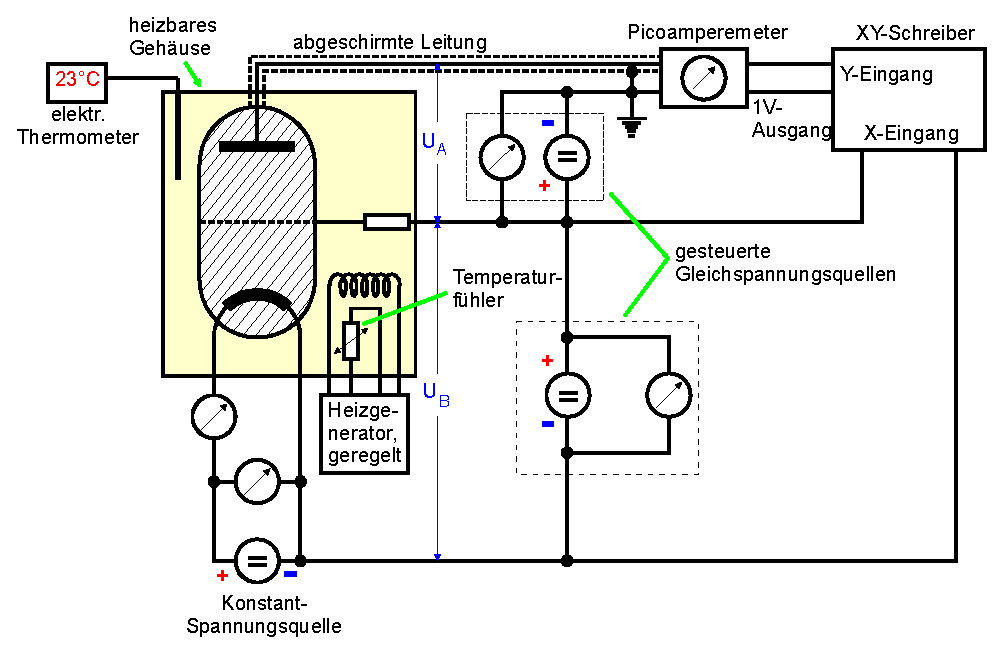
\includegraphics[width = 10 cm]{Aufbau.pdf}
    \caption{Aufbau der Apparatur \cite{ap601}.}
    \label{fig:AufbauMessung}
\end{figure}

Der Auffangstrom $I_{\text{A}}$, welcher nur sehr gering ist, misst man mit einem Picoamperemeter.
Die Franck-Hertz-Kurve wird mit Hilfe eines XY-Schreibers aufgezeichnet. Der X-Anschluss wird mit der Beschleunigungsspannung 
gespeist und die Auffängerspannung $U_{\text{A}}$ wird an den Y-Eingang geschlossen.